\documentclass{beamer}
% \usetheme[
% %%% options passed to the outer theme
% %    progressstyle=fixedCircCnt,   %either fixedCircCnt, movCircCnt, or corner
% %    rotationcw,          % change the rotation direction from counter-clockwise to clockwise
% %    shownavsym          % show the navigation symbols
%   ]{SDUsimple}
\usepackage{SDUtheme/beamerthemeSDUsimple}
% If you want to change the colors of the various elements in the theme, edit and uncomment the following lines
% Change the bar and sidebar colors:
%\setbeamercolor{SDUsimple}{fg=red!20,bg=red}
%\setbeamercolor{sidebar}{bg=red!20}
% Change the color of the structural elements:
%\setbeamercolor{structure}{fg=red}
% Change the frame title text color:
%\setbeamercolor{frametitle}{fg=blue}
% Change the normal text color background:
%\setbeamercolor{normal text}{fg=black,bg=gray!10}
% ... and you can of course change a lot more - see the beamer user manual.
\usepackage{color}
\usepackage{float}
\usepackage{dsfont}                         % Enables double stroke fonts
\usepackage{bm}
\usepackage[utf8]{inputenc}
\usepackage[english]{babel}
\usepackage[T1]{fontenc}
\usepackage{listings}
\usepackage{todonotes}
\usepackage{color}
% \usepackage{listings}
% \usepackage[ruled,vlined]{algorithm2e}
% Or whatever. Note that the encoding and the font should match. If T1
% does not look nice, try deleting the line with the fontenc.
\usepackage{helvet}
\usepackage{xmpmulti}
\usepackage{animate}
%\usepackage{movie15}
\usefonttheme{professionalfonts}

\newtheorem{algorithm}{Algorithm}
%\newtheorem{problem}{Problem}
\newtheorem{proposition}{Proposition}
% colored hyperlinks
\newcommand{\chref}[2]{%
  \href{#1}{{\usebeamercolor[bg]{SDUsimple}#2}}%
}

\title{Machine (or Reinforcement): Learning to assist vessel docking in extreme environments}
\subtitle{Bachelor defense}
%\date{\today}
\date{\today }

\author{
  \textbf{Anne-Charlotte Poulsen}
}

% - Give the names in the same order as they appear in the paper.
% - Use the \inst{?} command only if the authors have different
%   affiliation. See the beamer manual for an example

\institute[
%  {\includegraphics[scale=0.2]{SDU_segl}}\\ %insert a company, department or university logo
  SDU Robotics\\
  The Maersk Mc-Kinney Moller Institute\\
  University of Southern Denmark
] % optional - is placed in the bottom of the sidebar on every slide
{% is placed on the bottom of the title page
  SDU Robotics\\
  The Maersk Mc-Kinney Moller Institute\\
  University of Southern Denmark

  %there must be an empty line above this line - otherwise some unwanted space is added between the university and the country (I do not know why;( )
}

% specify a logo on the titlepage (you can specify additional logos an include them in
% institute command below
\pgfdeclareimage[height=0.5cm]{titlepagelogo}{SDUgraphics/SDU_logo_new} % placed on the title page
%\pgfdeclareimage[height=1.5cm]{titlepagelogo2}{SDUgraphics/SDU_logo_new} % placed on the title page
\titlegraphic{% is placed on the bottom of the title page
  \pgfuseimage{titlepagelogo}
%  \hspace{1cm}\pgfuseimage{titlepagelogo2}
}

\begin{document}
% the titlepage
{\SDUwavesbg%
\begin{frame}[plain,noframenumbering] % the plain option removes the header from the title page
  \titlepage
\end{frame}}
%%%%%%%%%%%%%%%%

% TOC
% \begin{frame}{Agenda}{\vphantom{(y}}
% \tableofcontents
% \end{frame}
%%%%%%%%%%%%%%%
\begin{frame}{Agenda}{\vphantom{(y}}
  %% Needed if you want to use table of content instead of itemize.
  % \section{Introduction}
  % \section{Reinforcement Learning}
  % \section{Simplified model}
  % \section{Results \& Discussion}
  % \section{Conclusion \& Future work}
  \begin{itemize}
    \item Quick introduction to the problem
    \item Reinforcement Learning
    \item Simplified model
    \item Results \& Discussion
    \item Conclusion \& Future work
  \end{itemize}
\end{frame}

\begin{frame}{Introduction}{The Vessel and the problem\vphantom{(y}}
  The issue is keeping the vessel stable enough to attach to the windmill during a storm.
\begin{columns}
    \begin{column}{0.48\textwidth}
      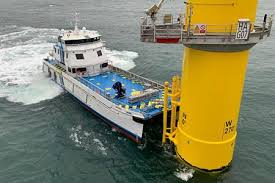
\includegraphics[width=1\textwidth]{images/docking_boat}
    \end{column}
    \begin{column}{0.48\textwidth}
        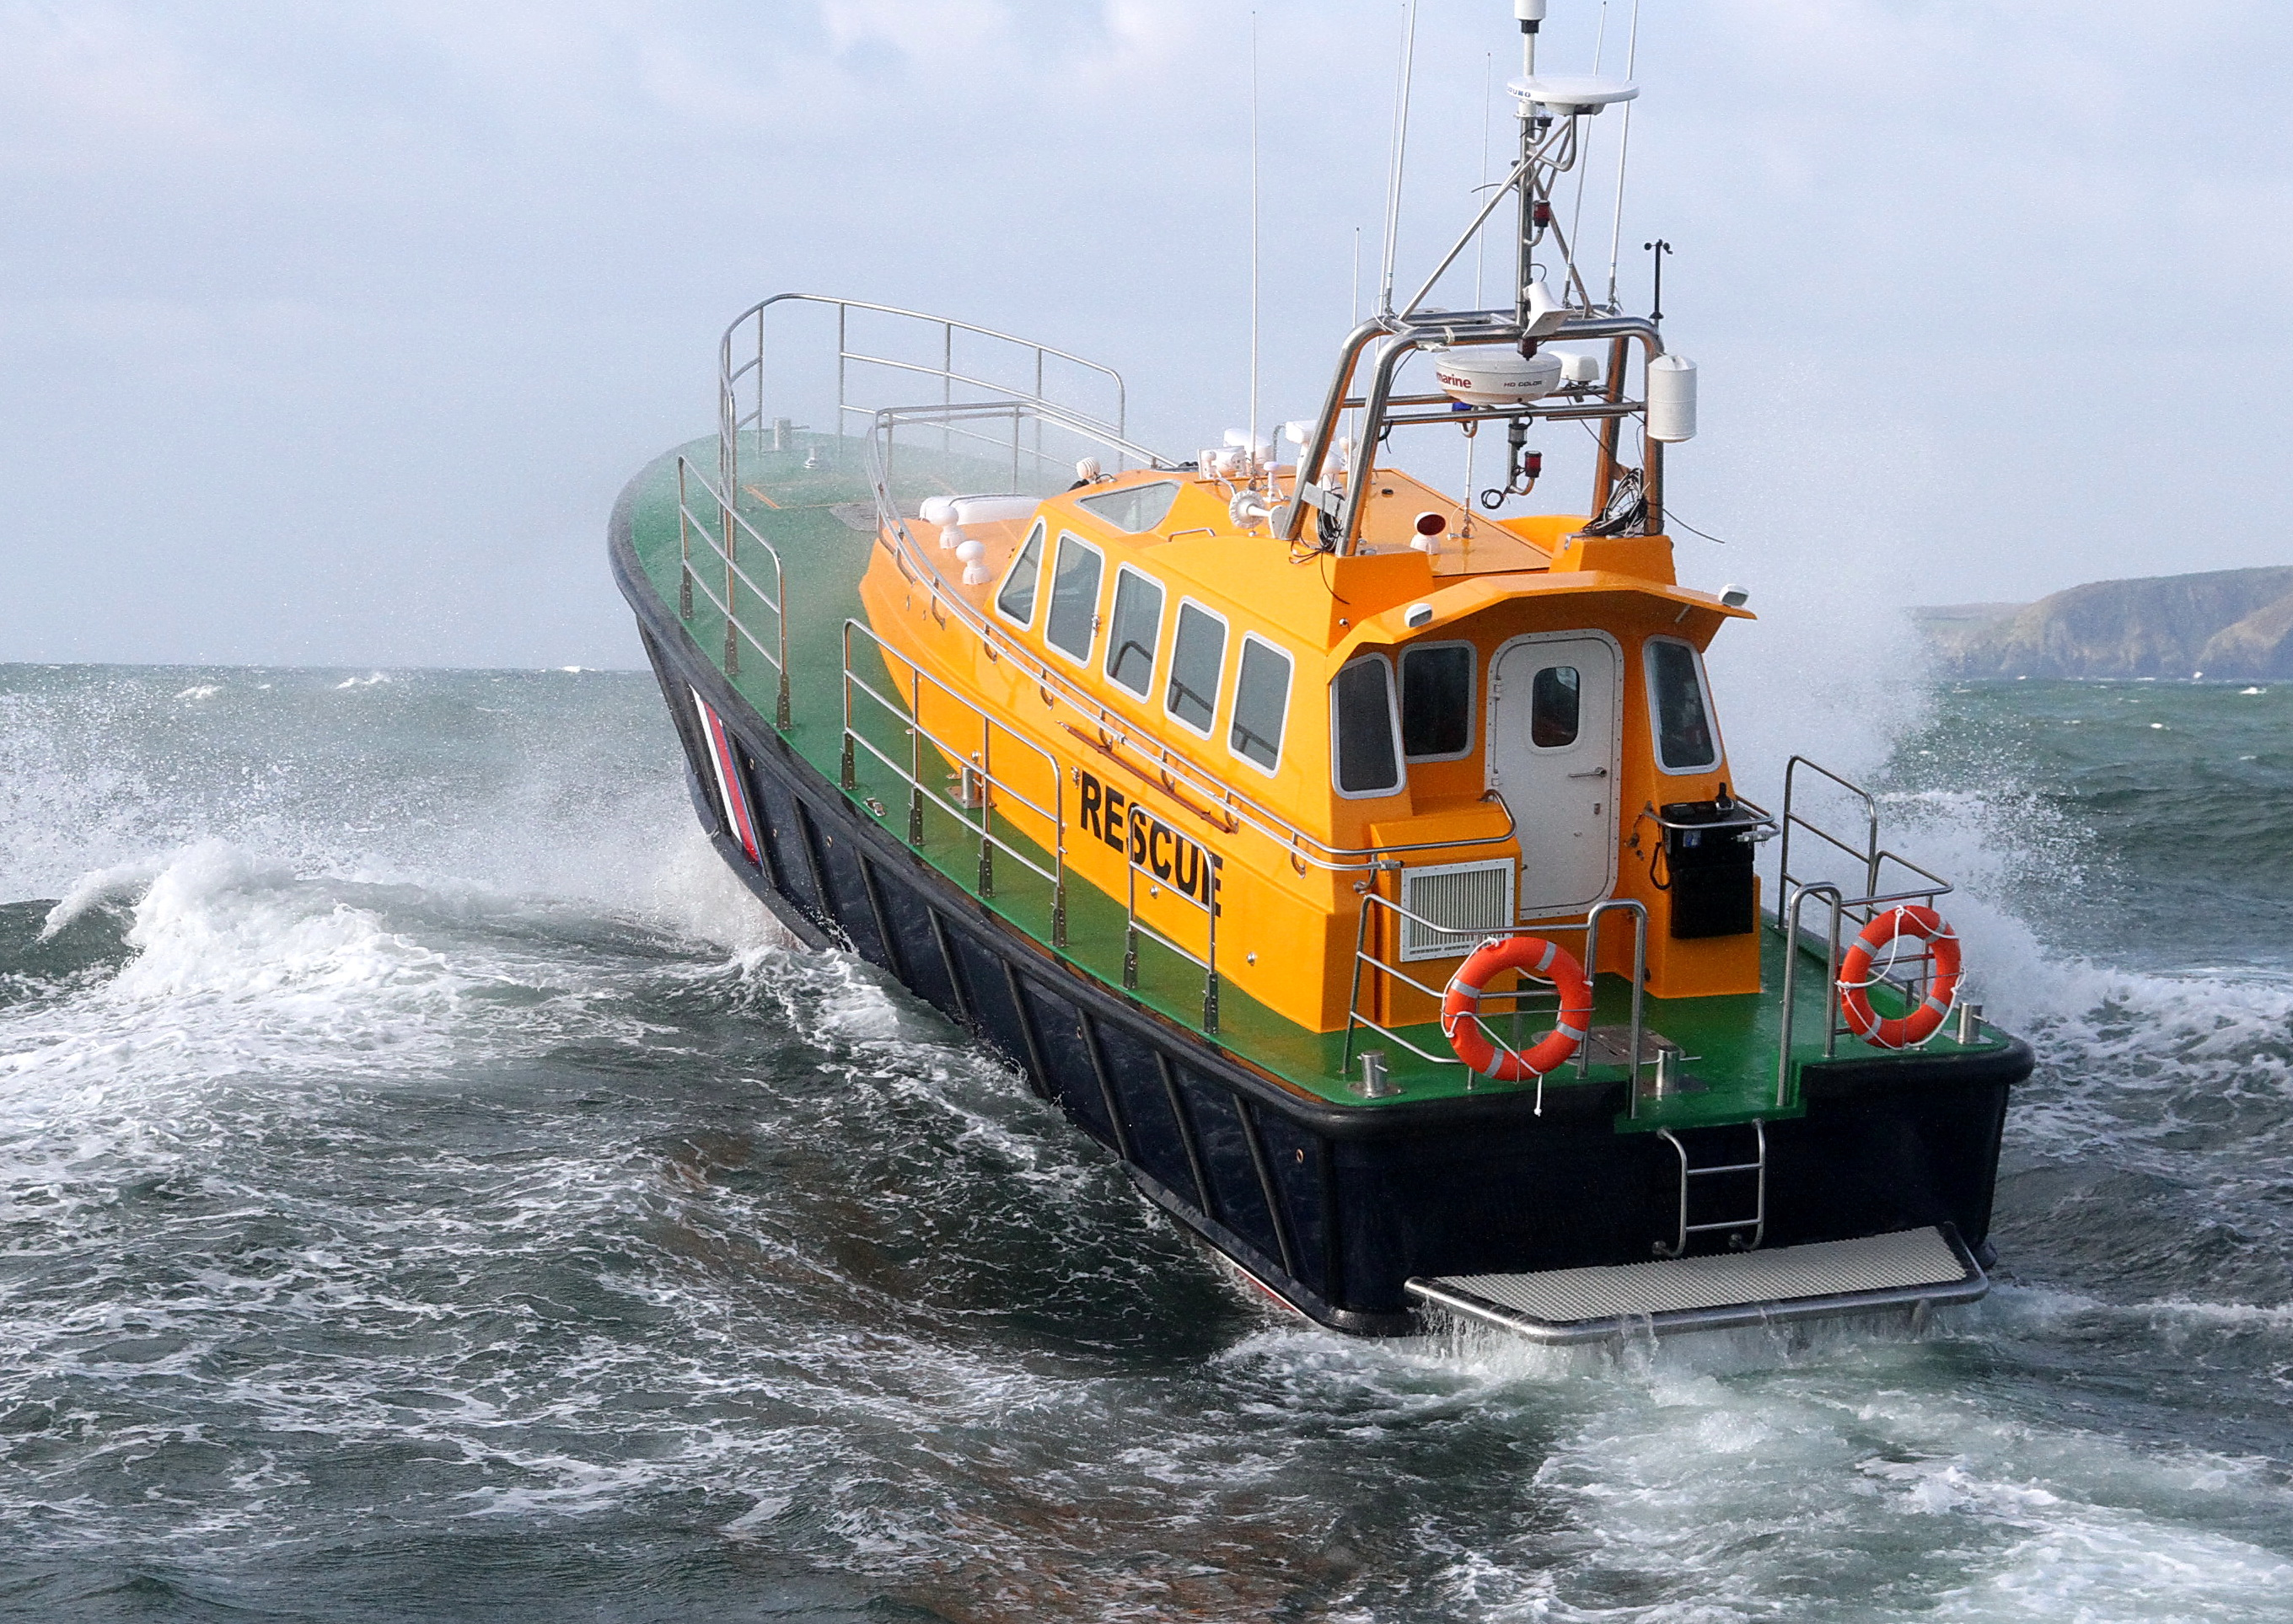
\includegraphics[width=1\textwidth]{images/boat2_storm}
    \end{column}
\end{columns}
\end{frame}


\begin{frame}{Introduction}{The problem and the solution\vphantom{(y}}
\vspace{-0.7em}
%\animategraphics[loop,controls,width=\linewidth]{300}{gifs/dacoma_frame_}{0001}{0300}
\end{frame}

\begin{frame}{Introductory}{Approach\vphantom{(y}}
\vspace{-0.7em}
Overview of the problem
\begin{itemize}
\item Vessel stabilizer
\item Why is a vessel stabilizer needed?
\item What is Dacoma's current solution?
\item The objective
\item {\color{blue}The approach}
\end{itemize}
\end{frame}



\begin{frame}{Reinforcement Learning}{Classic Reinforcement Learning \& Terminology\vphantom{(y}}
\vspace{-0.7em}

\begin{columns}
    \begin{column}{0.48\textwidth}
      \begin{itemize}
      \item Agent
      \item Environment
      \item States, Statespace, Actions \& Actionspace
      \item Reward and Reward function
      \item Policy
      \end{itemize}
    \end{column}
    \begin{column}{0.48\textwidth}
        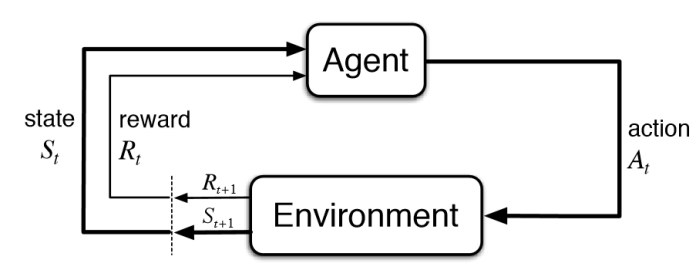
\includegraphics[width=1\textwidth]{images/rl_explained.jpg}
    \end{column}
\end{columns}
% Classic Reinforcement Learning (CRL)
% \begin{itemize}
%   \item Markov Decision Process (MDP)
%   \item Problem Review
%   \item Why CCRL does not fit on this problem
% \end{itemize}
\end{frame}

\begin{frame}{Reinforcement Learning}{Classic Reinforcement Learning \& Terminology\vphantom{(y}}
\vspace{-0.7em}
\begin{centering}
  Why does classic Reinforcement learning not work for this problem?
\end{centering}

\end{frame}

\begin{frame}{Reinforcement Learning}{The Policy gradient methods\vphantom{(y}}
\vspace{-0.7em}
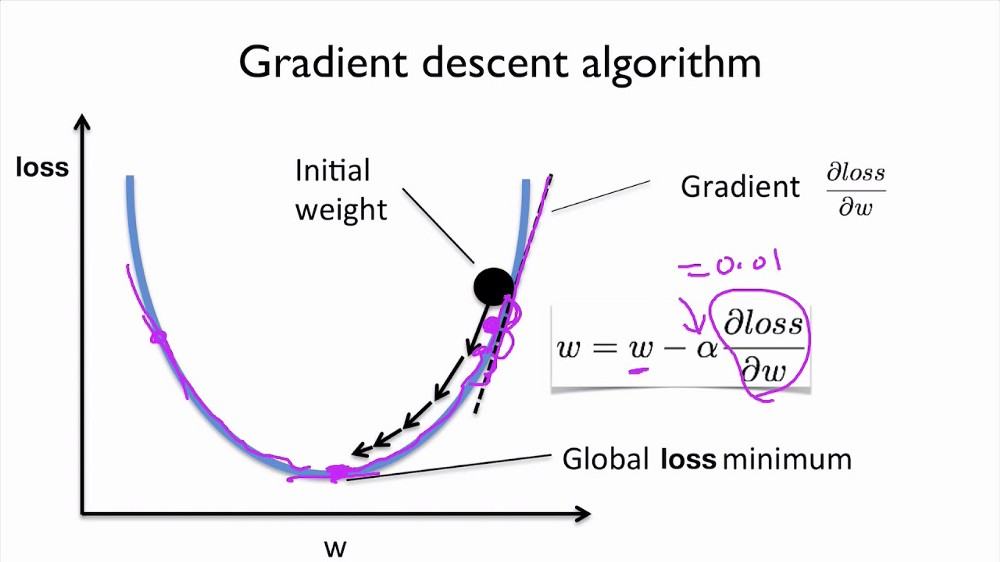
\includegraphics[width=1\textwidth]{images/gradient_descent.png}

What makes Policy gradient well-suited for this task? \\
\end{frame}

\begin{frame}{Reinforcement Learning}{The Neural Networks\vphantom{(y}}
\vspace{-0.7em}
        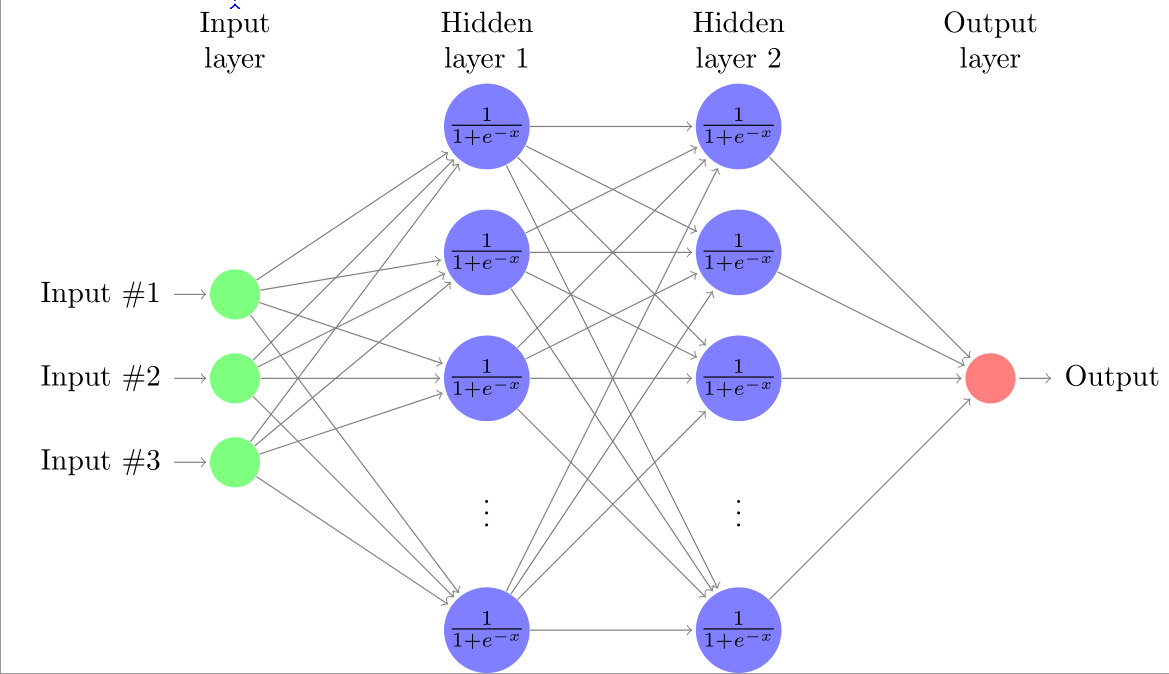
\includegraphics[width=1\textwidth]{images/NN_illu.png}

\end{frame}

\begin{frame}{Reinforcement Learning}{The Optimizer \vphantom{(y}}
\vspace{-0.7em}
\begin{columns}
    \begin{column}{0.48\textwidth}
        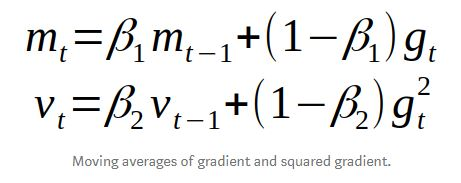
\includegraphics[width=1\textwidth]{images/adam_unbiased.JPG}
    \end{column}
    \begin{column}{0.48\textwidth}
        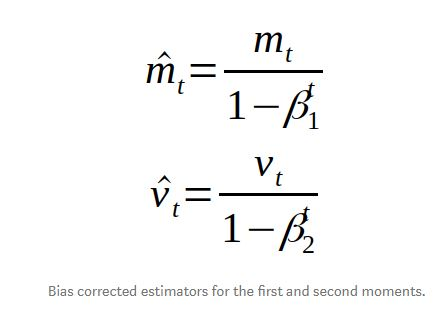
\includegraphics[width=1\textwidth]{images/adam_bias.JPG}
    \end{column}
\end{columns}
\end{frame}

\begin{frame}{Reinforcement Learning}{The Optimizer \vphantom{(y}}
\vspace{-0.7em}
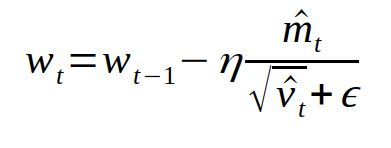
\includegraphics[width=1\textwidth]{images/adam_update.JPG}

\end{frame}

\begin{frame}{Reinforcement Learning}{The approach - finite differences method\vphantom{(y}}
\vspace{-0.7em}
Central difference ?
$$\Delta _{h}[f](x)=f\left(x+{\tfrac {1}{2}}h\right)-f\left(x-{\tfrac {1}{2}}h\right)$$

%
% \begin{algorithm}[H]
% \SetAlgoLined
% \KwResult{returns the reward and updates the gradient vector}
%  input: policy weights $\theta_h$ \& gradient vector $g_y$\;
%  \for{for n=0 to 500 do}{\;
%   generate policy variation $\epsilon \theta_n$\;
%   estimate $\dot{J_{+\epsilon}}_n \approx J(\theta_h + \frac{1}{2}\epsilon \theta_n)$ from roll-out \;
%   estimate  $\dot{J_{-\epsilon}}_n \approx J(\theta_h - \frac{1}{2}\epsilon \theta_n)$ from roll-out\;
%   compute $\Delta \dot{J_i} \approx J(\theta_h + \frac{1}{2}\epsilon  \theta_n)  - J(\theta_h - \frac{1}{2}\epsilon  \theta_n)$\;
%   compute $r += \frac{1}{2} (\cdot J_{+\epsilon}}_n + J_{-\epsilon}}_n) $\;
%  }
%  compute gradient estimate vector $g_y = (\epsilon \Theta ^T\epsilon \Theta)^{-1}\epsilon \Theta ^T \Delta \dot{J}$\;
%  return reward $R_{PD} = \frac{r}{500}$\;
%  \caption{Policy Gradient Estimation using finite differences altered to fit the actual implementation}
%  \label{al::alg2}
% \end{algorithm}
\end{frame}

\begin{frame}{Reinforcement Learning}{The approach - Implementation specifics\vphantom{(y}}
\vspace{-0.7em}
\begin{itemize}
  \item {\color{blue}Reward \& Reward Function}
\end{itemize}
\end{frame}


\begin{frame}{Simplified Model}{Intro\vphantom{(y}}
\vspace{-0.7em}
Using Archimedes principle and a adjustable air keel works to our advantages, the boat can stabilize itself.
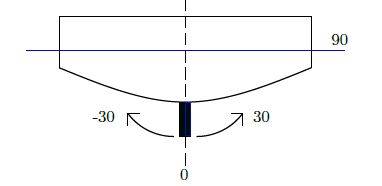
\includegraphics{images/boat_keel.JPG}
\end{frame}

\begin{frame}{Simplified Model}{Bouyancy \vphantom{(y}}
\vspace{-0.7em}
\begin{figure}
  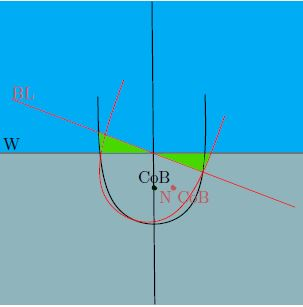
\includegraphics[scale=0.7]{images/boat_b.JPG}
\end{figure}

\end{frame}

\begin{frame}{Simplified Model}{Boat modelling \vphantom{(y}}
\vspace{-0.7em}
\begin{itemize}
  \item {\color{blue}Boat modelling}
\end{itemize}
\begin{figure}
  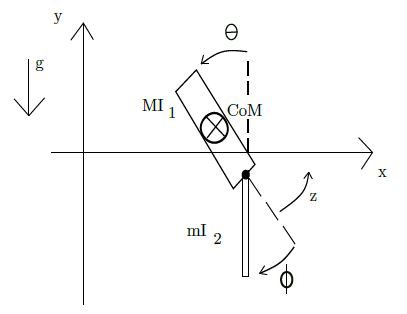
\includegraphics[scale=0.7]{images/link_model.JPG}
\end{figure}
\end{frame}

\begin{frame}{Simplified Model}{The model \vphantom{(y}}
\vspace{-0.7em}
$$
  M(q)\dot{\dot{q}} + C(q,\dot{q})\dot{q} + G(g) k_{\epsilon}q + B_F \dot{q}  = \Gamma
$$
\footnotesize{
where M(q) is the inertia matrix, C(q,$\dot{q}$) are the Coriolis terms, G(q) is the gravity vector, $k_{eqsilon}$ is a matrix with the elastic constants, $B_F$ is the friction terms and $\Gamma$ is the vector of generalized external forces applied, i.e $\Gamma ^\tau = [0,0,0,z]$.}

Limitations?
\end{frame}

\begin{frame}{Results \& Discussion }{Training \vphantom{(y}}
\vspace{-0.7em}
{\color{blue}Training and testing settings and limitations}

\footnotesize{\begin{itemize}
  \item 500 rollouts, 200 iterations and two simulations
  \item Random generated bias values
  \item Angle limitations for the keel ($\pm 40$) and boat ($\pm 30 $)
  \item Angles randomly generated to be between $\pm 25$.
  \item Activation function = Leaky ReLU
  \item Central finite difference, $\epsilon = 0.1262$
  \item Adam as optimizer
  \item Stopping criteria is $\pm 1 \degree$
\end{itemize}}
\end{frame}

\begin{frame}{Results \& Discussion }{Tuning \vphantom{(y}}
\vspace{-0.7em}
{\color{blue}Tuning hyperparameters}

\footnotesize{\begin{itemize}
  \item NN architecture
  \item Learning rate
\end{itemize}}

\begin{table}[h]
\centering
\begin{tabular}{l | l | l | 1}
 & HL = 1 \& NoN = 8 (HL1) & HL = 2 \& NoN = 8,4 (HL2) & HL = 2 \& NoN = 8,8 (HL3) \\
\hline
LR & 0.1 & 0.01 & 0.001 \\
LR & 0.2 & 0.02 & 0.002 \\
LR & 0.5 & 0.05 & 0.005
\end{tabular}
\caption{Displays the different learning rates tested with the three different architectural choices.}
\end{table}\\
\end{frame}

\begin{frame}{Results \& Discussion }{Tuning - NN architecture\vphantom{(y}}
\vspace{-0.7em}
\begin{figure}
  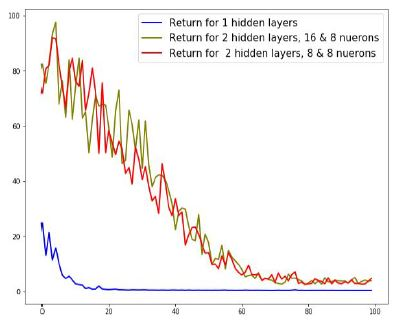
\includegraphics[scale=0.7]{images/lr_low_a.JPG}
  \caption{Learning rate: 0.001}
\end{figure}
\end{frame}

\begin{frame}{Results \& Discussion }{Tuning - NN architecture\vphantom{(y}}
\vspace{-0.7em}
\begin{figure}
  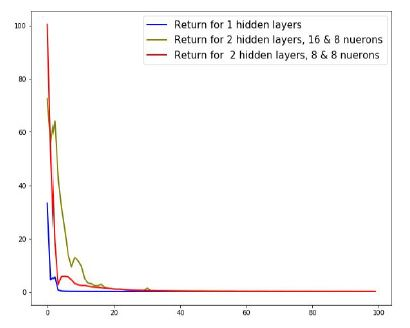
\includegraphics[scale=0.7]{images/lr_med_a.JPG}
  \caption{Learning rate: 0.01}
\end{figure}
\end{frame}

\begin{frame}{Results \& Discussion }{Tuning - NN architecture\vphantom{(y}}
\vspace{-0.7em}
\begin{figure}
  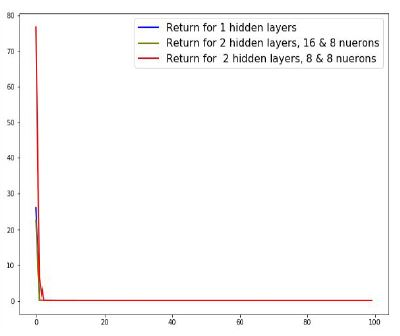
\includegraphics[scale=0.7]{images/lr_high_a.JPG}
  \caption{Learning rate: 0.1}
\end{figure}
\end{frame}

\begin{frame}{Results \& Discussion }{Tuning - Learning rates\vphantom{(y}}
\vspace{-0.7em}
\begin{figure}
  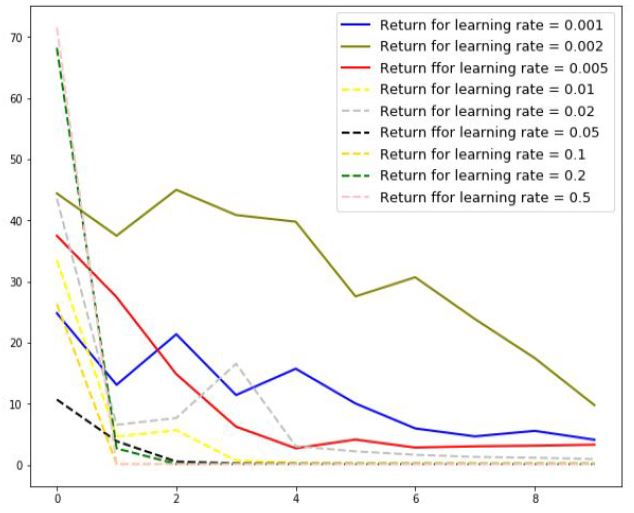
\includegraphics[scale=0.5]{images/lr_cropped_0_10.JPG}
  \caption{All learning rates cropped from 0 to 10 iterations}
\end{figure}
\end{frame}

\begin{frame}{Results \& Discussion }{Tuning - Learning rates\vphantom{(y}}
\vspace{-0.7em}
\begin{figure}
  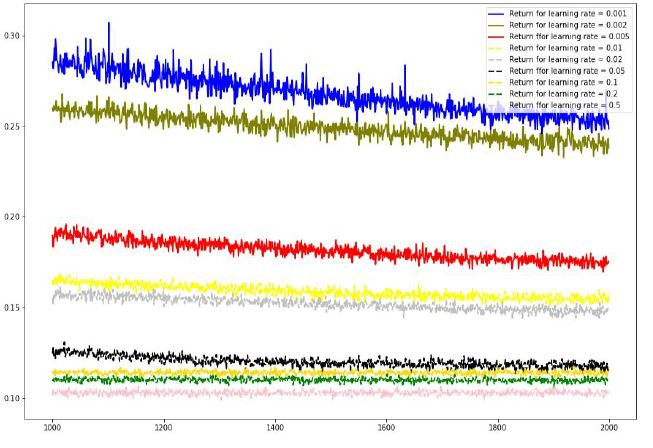
\includegraphics[scale=0.5]{images/lr_cropped_end.JPG}
  \caption{All learning rates cropped from 1000 to 2000 iterations}
\end{figure}
\end{frame}

\begin{frame}{Results \& Discussion }{Tuning - Learning rates\vphantom{(y}}
\vspace{-0.7em}
\begin{figure}
  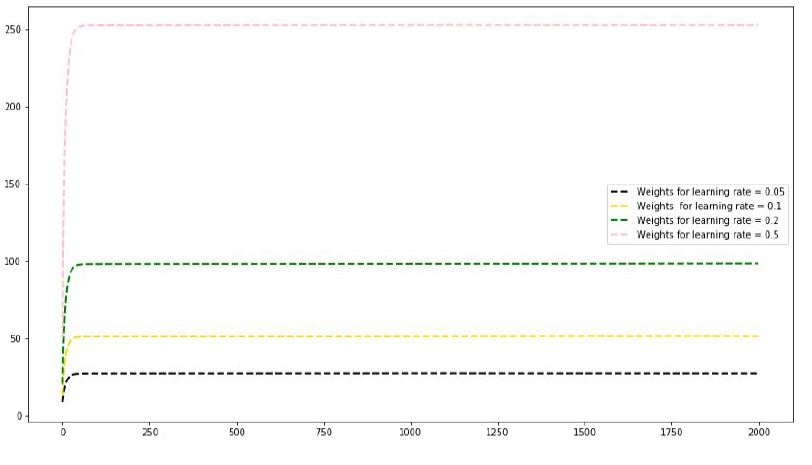
\includegraphics[scale=0.5]{images/weights.JPG}
  \caption{Shows the weights from chosen learning rates}
\end{figure}
\end{frame}


\begin{frame}{Results \& Discussion }{Tests and results \vphantom{(y}}
\vspace{-0.7em}
\begin{table}
\centering
\begin{tabular}{ l | l}
$\phi$ & $\theta$ \\
\hline
 $0^{\circ}$ & $\pm 20^{\circ}$ \\
 $0^{\circ}$ & $\pm 15^{\circ}$ \\
 $0^{\circ}$ & $\pm 10^{\circ}$ \\
 $\pm 5^{\circ}$ & $\pm 20^{\circ}$ \\
 $\pm 5^{\circ}$ & $\pm 15^{\circ}$ \\
 $\pm 5^{\circ}$ & $\pm 10^{\circ}$ \\
 $\pm 10^{\circ}$ & $\pm 20^{\circ}$ \\
 $\pm 10^{\circ}$ & $\pm 15^{\circ}$ \\
 $\pm 10^{\circ}$ & $\pm 10^{\circ}$ \\
 $\pm 15^{\circ}$ & $\pm 20^{\circ}$ \\
 $\pm 15^{\circ}$ & $\pm 15^{\circ}$ \\
 $\pm 15^{\circ}$ & $\pm 10^{\circ}$ \\
 $\pm 20^{\circ}$ & $\pm 20^{\circ}$ \\
 $\pm 20^{\circ}$ & $\pm 15^{\circ}$ \\
 $\pm 20^{\circ}$ & $\pm 10^{\circ}$
\end{tabular}
\end{table}
\end{frame}

\begin{frame}{Results \& Discussion }{Tests and results \vphantom{(y}}
\vspace{-1.4em}
\begin{table}
\centering
\begin{tabular}{l | l | l | 1 | 1}
Test \# & $\phi$ & $\theta$ & CC without torque limit & CC with torque limit \\
\hline
1 & 0$^{\circ}$ & -20$^{\circ}$ & 0.1345 & 0.9  \\
2 & 0$^{\circ}$ & -15$^{\circ}$ & 0.1341 & 0.73 \\
3 & 0$^{\circ}$ & -10$^{\circ}$ & 0.1320 &  0.48\\
4 & 5$^{\circ}$ & -20$^{\circ}$ & 0.1423 & 0.9 \\
5 & 5$^{\circ}$ & -15$^{\circ}$ & 0.1395 & 0.74 \\
6 & 5$^{\circ}$ & -10$^{\circ}$ & 0.1350 & 0.48 \\
7 & 10$^{\circ}$ & -20$^{\circ}$ & 0.1384 & 0.9 \\
8 & 10$^{\circ}$ & -15$^{\circ}$ & 0.1365 & 0.73 \\
9 & 10$^{\circ}$ & -10$^{\circ}$ & 0.1324 & 0.48 \\
10 & 15$^{\circ}$ & -20$^{\circ}$ & 0.1348 &  0.74 \\
11 & 15$^{\circ}$ & -15$^{\circ}$ & 0.1384 & 0.73 \\
12 & 15$^{\circ}$ & -10$^{\circ}$ & 0.1354 & 0.73 \\
13 & 20$^{\circ}$ & -20$^{\circ}$ & 0.½320 & 0.91 \\
14 & 20$^{\circ}$ & -15$^{\circ}$ & 0.1315 & 0.91 \\
15 & 20$^{\circ}$ & -10$^{\circ}$ & 0.1321 & 0.9
\end{tabular}
\end{table}
\end{frame}

\begin{frame}{Conclusion \& Future Works }{Conclusion \vphantom{(y}}
\vspace{-0.7em}

\begin{itemize}
  \item Use reinforcement to apply a torque to the air keel in order to keep the vessel stable.
  \item Derived a simplified model for simulation use.
  \item Trained and agent and found the best policy using the simplified modeled
  \item Added a mock limitation on the amount of torque which the agent could apply.
  \item Works well, maybe even a bit too well?
\end{itemize}
\end{frame}

\begin{frame}{Conclusion \& Future Works }{Future works \vphantom{(y}}
\vspace{-0.7em}
\begin{itemize}
  \item Torque limitations
  \item A model that includes the proper effect of Dacoma's air keel
  \item Adding waves to the model/training the model out in the sea
\end{itemize}
\end{frame}

\end{document}
